\documentclass[10pt]{beamer}

\usepackage{xeCJK}
\setCJKmainfont{Droid Sans Fallback}
\usepackage{booktabs}
\usepackage[table]{xcolor}
\usepackage{tikz}
\usetikzlibrary{arrows.meta,positioning}
\usepackage{helvet}
\renewcommand{\familydefault}{\sfdefault}
\definecolor{accent}{rgb}{0.05, 0.35, 0.75}

\setbeamertemplate{navigation symbols}{}
\setbeamertemplate{footline}[frame number]
\setbeamercolor{structure}{fg=accent}
\setbeamercolor{frametitle}{fg=black}
\setbeamercolor{block title}{fg=white, bg=accent}
\setbeamercolor{block body}{bg=accent!8}
\hypersetup{colorlinks=true, urlcolor=accent}

\newcommand{\pipelinefig}{%
  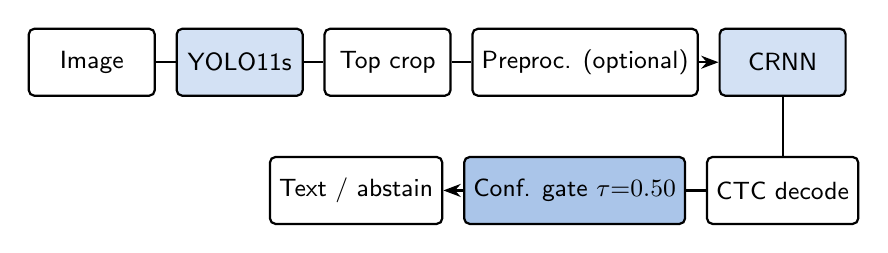
\begin{tikzpicture}[
    node distance=0.55cm and 0.25cm,
    box/.style={draw, thick, rounded corners=2pt, minimum width=1.6cm,
               minimum height=0.85cm, align=center, font=\small},
    model/.style={box, fill=accent!18},
    gate/.style={box, fill=accent!35},
    arr/.style={-{Stealth[length=2.2mm]}, thick}
  ]
  \node[box] (img) {Image};
  \node[model, right=of img] (det) {YOLO11s};
  \node[box, right=of det] (crop) {Top crop};
  \node[box, right=of crop] (pre) {Preproc. (optional)};
  \node[model, right=of pre] (ocr) {CRNN};
  \node[box, below=0.75cm of ocr] (ctc) {CTC decode};
  \node[gate, left=of ctc] (gate) {Conf. gate $\tau{=}0.50$};
  \node[box, left=of gate] (txt) {Text / abstain};
  \draw[arr] (img) -- (det) -- (crop) -- (pre) -- (ocr);
  \draw[arr] (ocr) -- (ctc) -- (gate) -- (txt);
  \end{tikzpicture}%
}

\begin{document}

% 1 ---------------------------------------------------------------
\begin{frame}[plain]
\begin{center}
\vspace*{2cm}
{\LARGE\bfseries License Plate Detection and\\ Recognition on CCPD2019}\\[1.0em]
Mikhail Krylov \(\cdot\) Andrei Polevoi \\[0.2em]
Maximilian Mifsud Bonici \(\cdot\) Evgenii Khovalyg\\[0.5em]
10 November 2026
\end{center}
\end{frame}

% 2 ---------------------------------------------------------------
\begin{frame}{Plan}
\begin{block}{Question}
Do these changes improve end-to-end plate recognition?
\end{block}
\vspace{0.6em}
\begin{itemize}
  \item Task: detect and read Chinese license plates
  \item Baseline: frozen YOLO11s detector + EasyOCR
  \item Upgrade 1: fine-tune the detector on CCPD2019
  \item Upgrade 2: replace EasyOCR with a task-specific CRNN
\end{itemize}
\end{frame}

% 2b --------------------------------------------------------------
\begin{frame}{Baselines}
\begin{columns}
  \column{0.5\textwidth}
  \textbf{Detection: frozen YOLO11s}
  \begin{itemize}
    \item Pretrained plate detector, 640\,px, top-score box only
    \item Weights \texttt{license-plate-finetune-v1s.pt}
  \end{itemize}
  \column{0.5\textwidth}
  \textbf{Recognition: EasyOCR}
  \begin{itemize}
    \item General-purpose OCR engine
    \item No Chinese plate prior
  \end{itemize}
\end{columns}
\vspace{0.6em}
\end{frame}

% 3 ---------------------------------------------------------------
\begin{frame}{CCPD2019}
\begin{center}
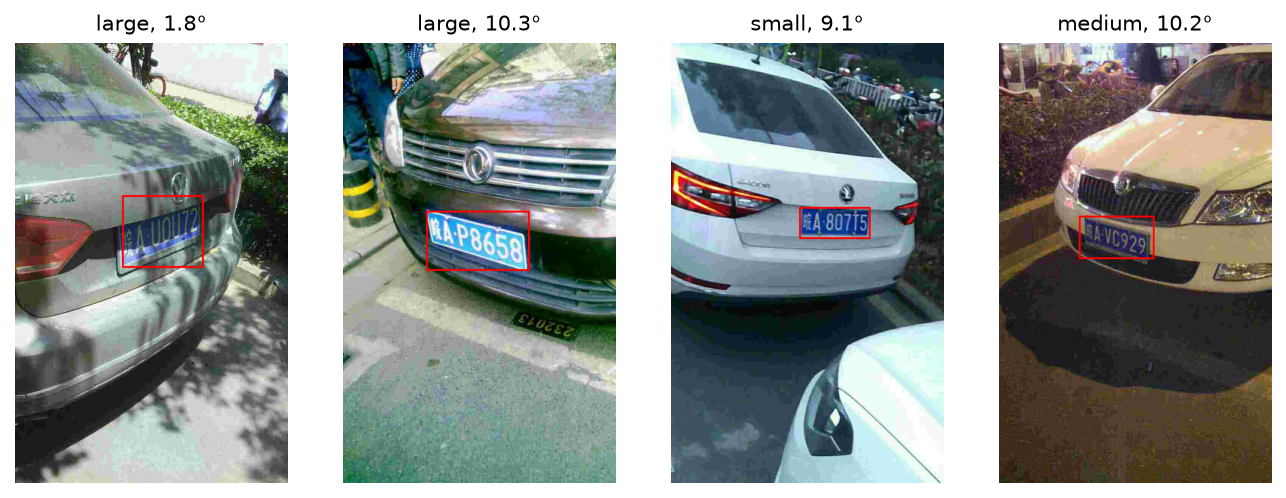
\includegraphics[width=0.92\textwidth]{../figures/ccpd_samples.png}
\end{center}
\vspace{0.5em}
\end{frame}

% 4 ---------------------------------------------------------------
\begin{frame}{Data Preparation}
\begin{columns}
  \column{0.52\textwidth}
  \textbf{The dataset}
  \begin{itemize}
    \item 352k images
    \item Box, tilt angles and plate text encoded in the file name
  \end{itemize}
  \column{0.48\textwidth}
  \textbf{Our subset}
  \begin{itemize}
    \item Stratified sampling by plate size and tilt angle
    \item 5,000 images
    \item Train / Test / Validation split: 3,500 / 700 / 800
  \end{itemize}
\end{columns}
\vspace{0.6em}
\begin{block}{Alphabet}
Province character $+$ latin letter $+$ 5 alphanumeric characters; 7 characters per plate.

Training alphabet is 58 characters: 24 province characters $+$ 10 digits $+$ 24 latin letters (I and O excluded).
\end{block}
\end{frame}

% 4b ---------------------------------------------------------------
\begin{frame}{Stratification strategy}
\begin{block}{Goal}
Preserve the source distribution of plate size and tilt angle: results reflect real conditions, not an easy subset.
\end{block}
\vspace{0.4em}
\begin{columns}
  \column{0.55\textwidth}
  \textbf{Strata}
  \begin{itemize}
    \item Plate height $\times$ tilt
    \item Quotas proportional to stratum size
    \item Split 3,500 / 700 / 800 assigned within strata, \emph{before} scale variants
  \end{itemize}
  \column{0.45\textwidth}
  \textbf{Scale variants}
  \begin{itemize}
    \item 1.0 / 0.75 / 0.5 per image
    \item 15,000 variants (10,500 / 2,100 / 2,400)
  \end{itemize}
  \vspace{0.5em}
  \begin{block}{Bins}
    height $\approx$ 75 / 96 / 127\,px \newline
    Tilt $\approx$ 16 / 90 / 92
  \end{block}
\end{columns}
\end{frame}

% 4 ---------------------------------------------------------------
\begin{frame}{Pipeline}
\begin{center}
\pipelinefig
\end{center}
\vspace{0.7em}
\end{frame}

% 5b ------------------------------------------------------------
\begin{frame}{Pipeline}
\begin{itemize}
  \item \textbf{Detection} is single-class YOLO11s at 640\,px. Only the top-score box is kept
  \item \textbf{Crop} is axis-aligned rectangle, no padding, no tilt correction
  \item \textbf{Recognition}: CRNN on image scaled to 48$\times$256 canvas with aspect-preserving fit and padding; CTC over 58 characters
  \item \textbf{Confidence} per character is max probability in CTC decoding run; $\tau{=}0.50$
\end{itemize}
\end{frame}



% 5 ---------------------------------------------------------------
\begin{frame}{Detection: fine-tune YOLO11s on the task}
\begin{itemize}
  \item Single class: license plate
  \item 640\,px input, batch 16, AdamW, lr 0.002
  \item 3,500 original-scale images, 24 epochs
  \item Best checkpoint by validation mAP@0.5 (epoch 4)
\end{itemize}
\end{frame}

% 8a ---------------------------------------------------------------
\begin{frame}{Preprocessing}
\begin{itemize}
  \item Three modes: \texttt{none} / grayscale $+$ CLAHE (clip 2.0, 8$\times$8) / Canny
  \item Applied at inference time, after the crop and before the recognizer
  \item The CRNN trains on raw crops, so any other mode is a distribution shift away from training
\end{itemize}
\end{frame}

% 6 ---------------------------------------------------------------
\begin{frame}{Recognition: CRNN replaces EasyOCR}
\begin{itemize}
  \item CNN + bidirectional LSTM + CTC, 2.99M parameters, selected epoch 39
  \item Alphabet: 58 characters + CTC blank
  \item 3,500 crops, total for training 50 epochs
  \item No preprocessing by default, confidence threshold 0.50
\end{itemize}
\end{frame}


% 5b1 -------------------------------------------------------------
\begin{frame}{CTC decoding}
\begin{itemize}
  \item The CRNN emits, at each of 16 timesteps, a probability over 59 symbols (58 characters $+$ blank)
  \item Greedy CTC decode: collapse repeated symbols, then remove the blanks
  \item Per-character confidence is the maximum probability inside its decoding run
  \item These per-character confidences feed the plate-level mean used by the gate
\end{itemize}
\end{frame}

% 5c ------------------------------------------------------------
\begin{frame}{Confidence}
\begin{itemize}
  \item Each decoded character carries a probability (max over its CTC run)
  \item Plate score is mean of the character probabilities
  \item Threshold $\tau$ chosen \emph{on validation only}: sweep 0.50--0.99, maximize
        (accepted exact accuracy $+$ coverage $- 1$)
  \item At the selected $\tau = 0.50$ all 800 test plates pass (lowest mean confidence 0.52)
  \item Raising $\tau$ to 0.90 abstains 259 plates. This raises number of false negatives in P/R/F1
\end{itemize}
\end{frame}

% 7 ---------------------------------------------------------------
\begin{frame}{Fine-tuning the detector closes the end-to-end gap}
\begin{center}
\footnotesize
\begin{tabular}{lcccc}
\toprule
Config & mAP@0.5 & F1 & Char.\ acc. & Exact \\
\midrule
Frozen YOLO11s + EasyOCR & 0.9073 & 0.9167 & 0.3240 & 0 / 800 \\
CRNN, GT crops & -- & -- & 0.7593 & 267 / 800 \\
CRNN + frozen YOLO11s & 0.9073 & 0.9167 & 0.6710 & 148 / 800 \\
\rowcolor{accent!12}
CRNN + fine-tuned YOLO11s & 0.9949 & 0.9714 & 0.7661 & 296 / 800 \\
\bottomrule
\end{tabular}
\end{center}
\end{frame}



% 8 ---------------------------------------------------------------
\begin{frame}{Canny preprocessing destroys the signal}
\begin{center}
\small
\begin{tabular}{lc}
\toprule
Preprocessing (val.\ char.\ acc.) & CRNN \\
\midrule
None & \textbf{0.7558} \\
Grayscale + CLAHE & 0.7469 \\
Canny edge detection & 0.4575 \\
\bottomrule
\end{tabular}
\end{center}
\vspace{0.6em}
\begin{center}
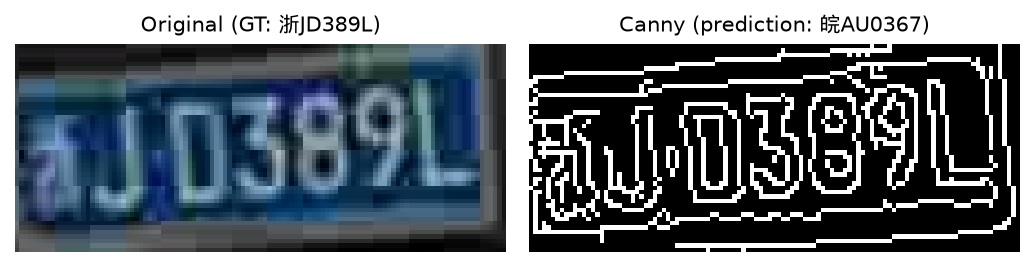
\includegraphics[width=0.95\textwidth]{../figures/failure_canny.png}
\end{center}
\end{frame}

% 9 ---------------------------------------------------------------
\begin{frame}{Accuracy holds across scales}
\begin{center}
\small
\begin{tabular}{lccc}
\toprule
Scale & Det.\ mAP@0.5 & Char.\ acc. & Exact plates \\
\midrule
1.00 & 0.9949 & 0.7661 & 296 / 800 \\
0.75 & 0.9966 & 0.7689 & 300 / 800 \\
0.50 & 0.9910 & 0.7174 & 241 / 800 \\
\bottomrule
\end{tabular}
\end{center}
\vspace{0.6em}
\begin{itemize}
  \item OCR accuracy doesn't depend on absolute size
\end{itemize}
\end{frame}

% 10 --------------------------------------------------------------
\begin{frame}{Failure analysis}
\begin{center}
\scriptsize
\begin{tabular}{lll}
\toprule
Model & Prediction (ground truth) & Likely reason \\
\midrule
EasyOCR & 苏E050R8 $\to$ 05oRo菲 & general OCR, no plate prior \\
CRNN & 皖AR1654 $\to$ 皖AR1564 & large crop shrunk to 48$\times$256 \\
Frozen YOLO11s & 51 of 800 missed & not trained on CCPD scenes \\
\bottomrule
\end{tabular}
\end{center}
\vspace{0.5em}
\begin{center}
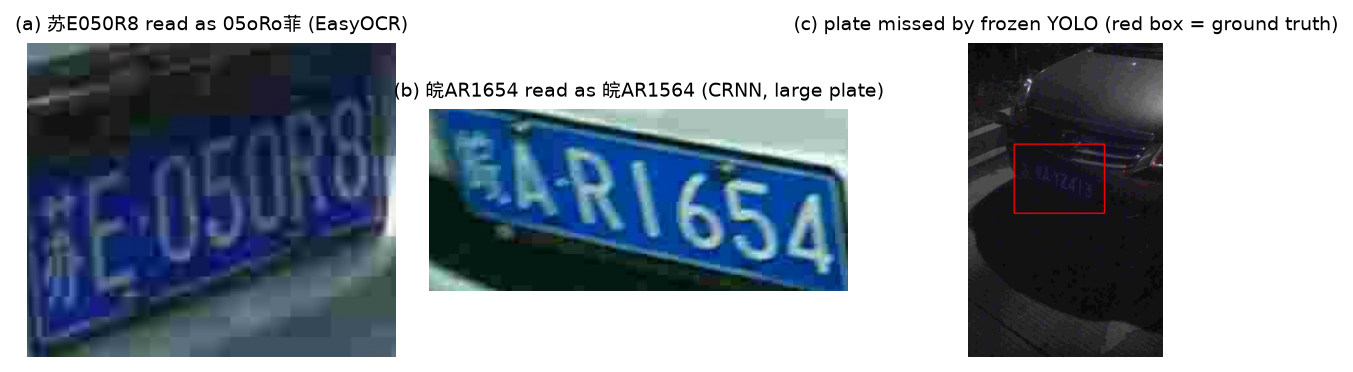
\includegraphics[width=0.95\textwidth]{../figures/failure_detection.png}
\end{center}
\end{frame}

% 11 --------------------------------------------------------------
\begin{frame}{Missed detections drive end-to-end error}
\begin{itemize}
  \item Frozen pipeline: 0.6710 vs.\ 0.7593 on GT crops
  \item Fine-tuning recovers the gap: 0.7661
  \item EasyOCR: 0 / 800 plates exact
  \item Fixed 48\(\times\)256 canvas: OCR is scale-invariant
  \item Next: larger inputs, size/tilt-balanced training
\end{itemize}
\end{frame}

% 12 --------------------------------------------------------------
\begin{frame}{Contributors}
\begin{itemize}
  \item Andrei Polevoi --- data and preprocessing
  \item Maximilian Mifsud Bonici --- detection
  \item Evgenii Khovalyg --- recognition
  \item Mikhail Krylov --- pipeline and evaluation
\end{itemize}
\end{frame}

% 13 --------------------------------------------------------------
\begin{frame}[plain]
\begin{center}
\vspace*{3cm}
{\LARGE Questions?}\\[1em]
{\large Thank you}\\[1.2em]
{\large \url{https://github.com/S1norin/inno-detecting-license-plates}}\\[0.5em]
{\small Demo video: \url{https://drive.google.com/file/d/1KBiiD-dvhvzsI7yWwDc7KqwM6jp585ez/view}}
\end{center}
\end{frame}

\end{document}
